\chapter{Analýza výkonnosti a obmedzení }


\section{Test výkonnosti knižníc Snap.svg.js a Raphael.js - animate()}

Vytvorila som test prostredníctvom webovej stránky, ktorá umožnuje robiť spustiteľné testy na rôznych platformách. Test sledoval počet operácií za sekundu. Čím viac operácií sa vykonalo, tým lepšie. Test sa spustil 100 krát za sebou najprv pre Raphael.js a potom pre Snap.svg.js. 
% \url{http://jsperf.com/snap-svg-raphael-js-animate}
 
% Benchmark.js v1.0.0 A robust benchmarking library that works on nearly all JavaScript platforms, supports high-resolution timers, and returns statistically significant results.


Test spočíva vo vytvorení kruhu na plátne na náhodných súradniciach a následne zanimovanie. Boli spustené animácie na kruh: 
\begin{itemize} \item náhodnej polohy x, y, 
\item zmeny farby výplne kruhu na náhodnú farbu, 
\item zmeny farby okraja na náhodnú farbu, 
\item zmeny šírky okraja na náhodnú hodnotu v rozsahu od 0 po 2. 
\end{itemize}
Testoval sa nasledovný kód: 
Pred spustením testu som si zadefinovala: 
\begin{lstlisting}[language = html]
<script src="https://rawgithub.com/adobe-webplatform/Snap.svg/master/dist/snap.svg.js"></script>
<script src="https://rawgithub.com/DmitryBaranovskiy/raphael/master/raphael.js"></script>

<div id="raphael"></div>
<svg id="snap"></svg>
<script>
var s = Snap('#snap');
var r = Raphael('raphael', 1000, 1000);
s.width=1000;
s.height=1000;
</script>
\end{lstlisting}

Testovací kód pre knižnicu Raphael.js:
\begin{lstlisting}
var raphaelCircle = r.circle(Math.random() * 1000, Math.random() * 1000, Math.random() * 10);
raphaelCircle.animate({
  x: Math.random() * 1000,
  y: Math.random() * 1000,
  fill: '#' + (Math.random() * 0xFFFFFF << 0).toString(16),
  stroke: '#' + (Math.random() * 0xFFFFFF << 0).toString(16),
  "stroke-width": Math.random() * 2,
}, 10);
\end{lstlisting}

Testovací kód pre knižnicu Snap.svg.js:
\begin{lstlisting}
var raphaelCircle = r.circle(Math.random() * 1000, Math.random() * 1000, Math.random() * 10);
raphaelCircle.animate({
  x: Math.random() * 1000,
  y: Math.random() * 1000,
  fill: '#' + (Math.random() * 0xFFFFFF << 0).toString(16),
  stroke: '#' + (Math.random() * 0xFFFFFF << 0).toString(16),
  "stroke-width": Math.random() * 2,
}, 10);
\end{lstlisting}


 \begin{figure}[H]
\centering
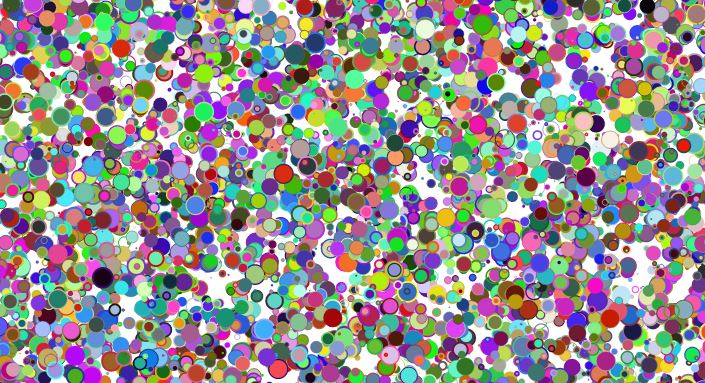
\includegraphics[width=0.7\linewidth]{obrazky/testovanieSnapVsRaphael.jpg}
\caption{Po spustení testovania výkonnosti knižníc Raphael.js vs Snap.svg.js - zobrazenie spusteních animácií}
\label{fig:podpora2}
\end{figure}


Na obrázku \ref{fig:podpora2} je výsledok animácie vykonaného testu. Test som spustila na viacerých platformách a webových prehliadačoch. Príklad výsledku pre konkrétny webový prehliadač je na obrázku \ref{fig:vyslMozila}



 \begin{figure}[H]
\centering
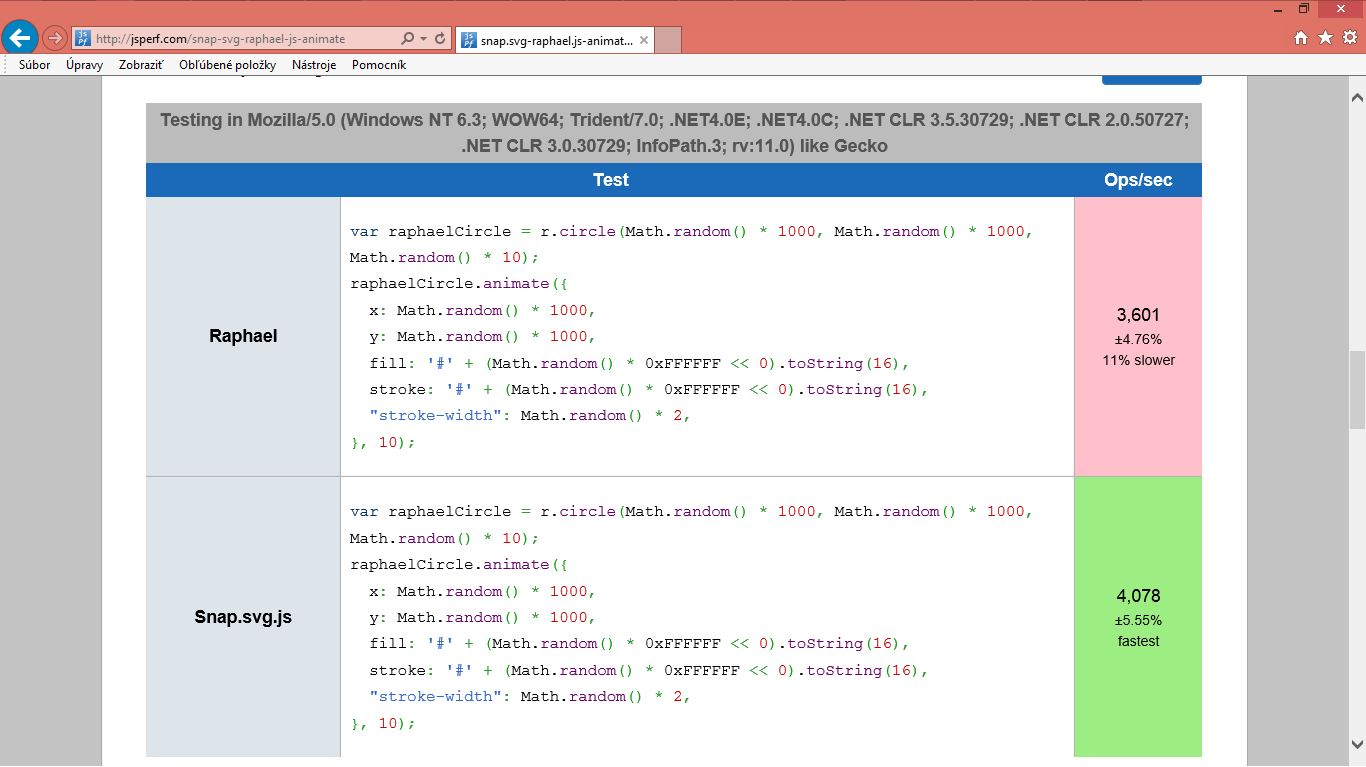
\includegraphics[width=0.7\linewidth]{obrazky/testovanieSnapVsRaphael2.jpg}
\caption{Po spustení testovania výkonnosti knižníc Raphael.js vs Snap.svg.js - výsledky pre konkrétny prehliadač}
\label{fig:vyslMozila}
\end{figure}

Výsledky testu sú nasledovné: 
\begin{itemize}
\item pre mobilné zariadenia a ich príslušné webové prehliadače sú v tabuľke \ref{tab:mobily}
\item pre súčastné a staršie verzie webových prehliadačoch, ktoré sú spustiteľné na počítačoch sú v tabuľke \ref{tab:pocitace}
\item pre staršie verzie webových prehliadačoch sú v tabuľke %\ref{tab:starsie}
\end{itemize}



\begin{table}[H]
	
\begin{center}

\begin{tabular}{|l|c|c|}
	\hline \textbf{Webový prehliadač} & \textbf{Raphael.js (ops/sec)} & \textbf{Snap.svg.js (ops/sec)} \\ 
	\hline Android 4.1.2 & 292 & 292 \\ 
	\hline Chrome 11.0.6996 & 1 283 & 1 283 \\ 
	\hline Chrome Mobile 42.0.2311 & 181 & 266 \\ 
	\hline Firefox Mobile 33.0 & 285 & 414 \\ 
	\hline 
\end{tabular} 
\end{center}

\caption{Výsledky testu pre mobilné zariadenia}
\label{tab:mobily}
	\end{table}

\begin{table}[H]
\begin{center}
		\begin{tabular}{|l|c|c|}
		\hline \textbf{Webový prehliadač} & \textbf{Raphael.js (ops/sec)} & \textbf{Snap.svg.js (ops/sec)} \\ 
		\hline Chrome 42.0.2311 & 2 753 & 2 171 \\ 
		\hline Epiphany 3.10.3 & 2 609 & 2 609 \\ 
		\hline Firefox 37.0. & 3 626 & 3 626 \\ 
	
			\hline IE 10.0 & 4 688 & 4 593 \\ 
			\hline IE 11 & 4 771 & 4 565 \\ 
			\hline Opera 25.0.1614 & 1 627 & 1 627 \\ 
			\hline Opera 29.0.1795 & 2 626 & 2 352 \\ 
			\hline Safari 5.1.7 & 3 249 & 3 050 \\ 
			\hline Iné & 1 432 & 1 427 \\ 
			\hline 
	
	\end{tabular} 
	
\end{center}
	\caption{Výsledky testu pre deskopové zariadenia}
	\label{tab:pocitace}
\end{table}

Súhrný graf výsledkov webových prehliadačov je na obrázku \ref{fig:graf}. Aritmetický priemer pre knižnicu Raphael.js je 2263.230769 a pre Snap.svg.js je 2175. Najlepšie výsledky dosiahol Internet Explorer verzia 11. 

 \begin{figure}[H]
\centering
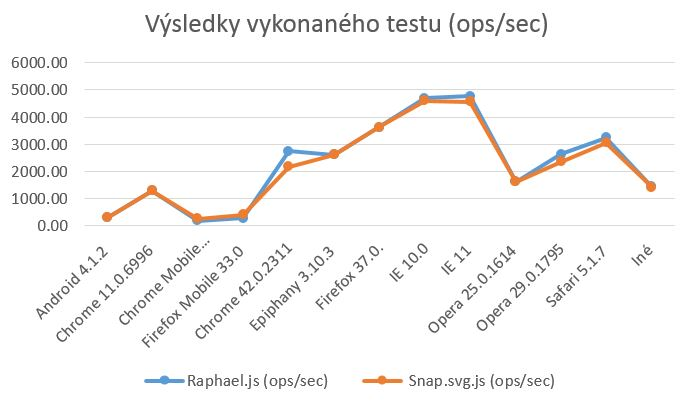
\includegraphics[width=0.9\linewidth]{obrazky/graf.JPG}
\caption{Graf výsledkov pre webové prehliadače}
\label{fig:graf}
\end{figure}



\section{Raphael.js vs Snap.SVG.js vs SVG.js - attr()}
Tento test bol zameraný na porovnanie výkonosti troch knižníc, ktoré umožňujú animáciu SVG. V teste sa vytváralo hmomadne kruhy s náhodnými hodnotami a následne po vykonaní iterácie sa vymazali. Iterácií prebehlo 100. 
%http://jsperf.com/raphael-vs-snapsvg-attr/7

multiple circles moved to the back

Kód testu: 

\begin{lstlisting}[language = html]
<script src="jquery.min.js"></script>
<script src="snap.svg.js"></script>
<script src="raphael.js"></script>
<script src="svg.js"></script>

<div id="raphael"></div>
<svg id="snap"></svg>
<svg id="svgjs"></svg>

<script>
var ncircs = 100;
var circs;

removecircs = function () {
    for (var i=0; i<circs.length; i++) {
      circs[i].remove();     }
   circs=[];};

var r = Raphael('raphael', 800, 600);
rapcirc = function () {
  var raphaelCircle = r.circle(400, 300, 150);
  raphaelCircle.attr({
    cx: raphaelCircle.attr('cx') + Math.random() * 50 - 25,
    cy: raphaelCircle.attr('cy') + Math.random() * 50 - 25
  }).toBack();
  circs.push(raphaelCircle);
  if (circs.length>=ncircs) removecircs();
};

var s = Snap('#snap');
s.width=800;
s.height=600;
snapcirc = function () {
  var snapCircle = s.circle(400, 300, 150);
  snapCircle.attr({
    cx: snapCircle.attr('cx') + Math.random() * 50 - 25,
    cy: snapCircle.attr('cy') + Math.random() * 50 - 25
  }).prependTo(s);
  circs.push(snapCircle);
  if (circs.length>=ncircs) removecircs();
};


var draw = SVG('svgjs').size(800, 600);
svgcirc = function () {
  var svgjsCircle = draw.circle(300).center(400, 300);
  svgjsCircle.attr({
    cx: svgjsCircle.attr('cx') + Math.random() * 50 - 25,
    cy: svgjsCircle.attr('cy') + Math.random() * 50 - 25
  }).back();
  circs.push(svgjsCircle);
  if (circs.length>=ncircs) removecircs();
};
</script>
 
\end{lstlisting}

Výsledok testu pre webový prehliadač je na obrázku~\ref{fig:graf2}

 \begin{figure}[H]
\centering
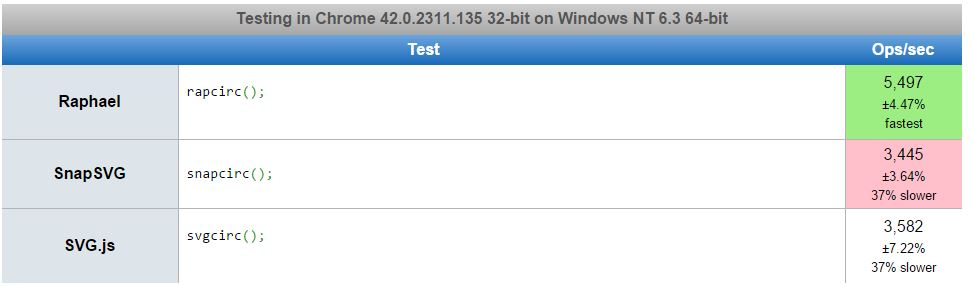
\includegraphics[width=0.7\linewidth]{obrazky/test2.JPG}
\caption{Test pre funkciu attr() pre webový prehliadač Chrome 42}
\label{fig:graf2}
\end{figure}





Výsledky vykonaných testov vo viacerých webových prehliadačoch sú na obrázku \ref{fig:graf3}.

 \begin{figure}[H]
\centering
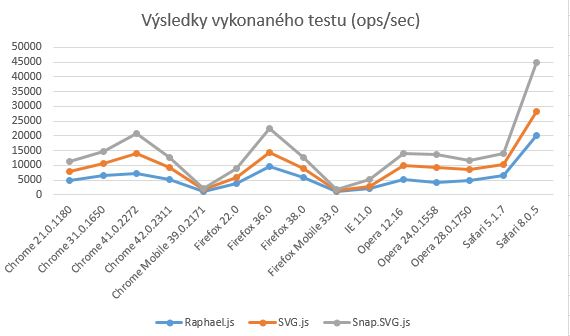
\includegraphics[width=0.9\linewidth]{obrazky/graf3.JPG}
\caption{Graf výsledkov pre webové prehliadače}
\label{fig:graf3}
\end{figure}


\begin{table}[H] \begin{center} \begin{tabular}{|l|c|c|c|} \hline \textbf{Webový prehliadač} & \textbf{Raphael.js} & \textbf{SVG.js} & \textbf{Snap.SVG.js}  \\ \hline Chrome 21.0.1180 & 4875 & 3147 & 3164  \\ \hline Chrome 41.0.2272 & 7268 & 6866 & 6589  \\ \hline Chrome 42.0.2311 & 5261 & 3976 & 3427  \\ \hline Chrome Mobile 39.0.2171 & 1073 & 746 & 398  \\ \hline Firefox 22.0 & 3946 & 1856 & 3158 \\ \hline Firefox 38.0 & 5835 & 2965 & 3783 \\ \hline Firefox Mobile 33.0 & 1156 & 309 & 426 \\ \hline IE 11.0 & 2272 & 724 & 2208 \\ \hline Opera 12.16  & 5239 & 4645 & 4092 \\ \hline Opera 24.0.1558 & 4150 & 5134 & 4461\\ \hline Opera 28.0.1750 & 4830 & 3827 & 3154 \\ \hline Safari 5.1.7 & 6709 & 3475 & 3919\\ \hline Safari 8.0.5 & 20226 & 8084 & 16438 \\ \hline \end{tabular} 
	
\end{center}
	\caption{Výsledky testu pre viaceré webové prehliadače (ops/sec)}
	\label{tab:test3}
\end{table}




\clearpage






\section{SVG vs Canvas}
%Počet objektov SVG 
%Zložitosť SVG - výpočtový výkon





%Sometimes there are outside influences that require a choice of technology that is, or is mostly, independent of functionality. For the question of using Canvas or SVG, there are two primary differentiators. Sometimes developer knowledge, skill set, and existing assets play a significant role into the choice of technologies. If a developer has deep knowledge of low level graphic APIs and limited knowledge of web technologies, the likely technology to choose is canvas.Also, performance is absolutely critical on high traffic websites. It is necessary to compare the performance characteristics of the two technologies. This might require the development of accessibility, custom styling, and more granular user interactions that do not come with canvas. It does not mean that canvas, though typically viewed as highly performant, is the obvious choice. The following graphs show the difference between of rendering time between SVG and Canvas objects.

Na obrázku \ref{fig:podpora23} sú zobrazené dva grafy, ktoré porovnavajú vlastnosti Canvas a SVG. 


Všeobecne platí, ak sa veľkosť obrazovky zvýši, plátno sa začne zmenšovať až na toľko pixelov, koľko je potrebné vykresliť. Pri SVG je to tak, ak sa počet objektov na obrazovke zvýši, tak začne neustále dané objekty pridávať do DOM.Tieto merania nie sú nevyhnutné presné a môžu sa zmeniť v závislosti od implementácie a platformy, hardvérovej akcelerácie grafiky. \cite{microsoft}


 \begin{figure}[H]
\centering
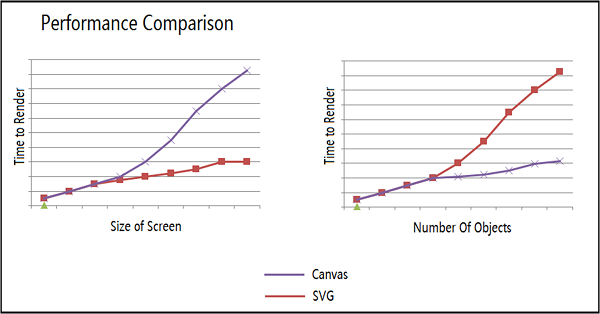
\includegraphics[width=1\linewidth]{obrazky/porovnanie}
\caption{Porovnanie výkonnosti Canvas vs. SVG}
\label{fig:podpora23}
\end{figure}






%Pre meranie výkonnosti vizualizácie grafických komponentov v reálnom čase zadefinujem v nasledujúce kritéria \begin{itemize}	\item počet komponentov, 	\item čas načítania stránky, 	\item čas vykonania zmeny atribútov v komponentoch.\end{itemize}Testy boli vykonané vo webovom prehliadači Chrome verzia 45 a Firefox verzia 40.  V teste boli použité nasledujúce navrhnuté komponenty:\begin{itemize}	\item teplomer, 	\item prečerpávacia stanica, 	\item trojcestný ventil, 	\item mapa Slovenska, 	\item prepravný pás. \end{itemize}Objekty boli v rovnakom zastúpení v jednom HTML súbore  v počtoch: 1,5,10,25, 50, 100.Ukážka testovacej situácie je na obrázku TODO SCREEN. A výsledky sú uvedené v tabuľke TODO TABULKA. \newpage Alebo vytvorim test -\url{http://jsperf.com/}- kde porovnam SVG smil animaciu s snap.svg.jsktore je v kapitole 4 - strana vtedy bola 20
